\documentclass[english,,man]{apa6}
\usepackage{lmodern}
\usepackage{amssymb,amsmath}
\usepackage{ifxetex,ifluatex}
\usepackage{fixltx2e} % provides \textsubscript
\ifnum 0\ifxetex 1\fi\ifluatex 1\fi=0 % if pdftex
  \usepackage[T1]{fontenc}
  \usepackage[utf8]{inputenc}
\else % if luatex or xelatex
  \ifxetex
    \usepackage{mathspec}
  \else
    \usepackage{fontspec}
  \fi
  \defaultfontfeatures{Ligatures=TeX,Scale=MatchLowercase}
\fi
% use upquote if available, for straight quotes in verbatim environments
\IfFileExists{upquote.sty}{\usepackage{upquote}}{}
% use microtype if available
\IfFileExists{microtype.sty}{%
\usepackage{microtype}
\UseMicrotypeSet[protrusion]{basicmath} % disable protrusion for tt fonts
}{}
\usepackage{hyperref}
\hypersetup{unicode=true,
            pdftitle={Principles for Describing or Explaining Process},
            pdfauthor={\ldots{}},
            pdfkeywords={\ldots{}.},
            pdfborder={0 0 0},
            breaklinks=true}
\urlstyle{same}  % don't use monospace font for urls
\ifnum 0\ifxetex 1\fi\ifluatex 1\fi=0 % if pdftex
  \usepackage[shorthands=off,main=english]{babel}
\else
  \usepackage{polyglossia}
  \setmainlanguage[]{english}
\fi
\usepackage{graphicx,grffile}
\makeatletter
\def\maxwidth{\ifdim\Gin@nat@width>\linewidth\linewidth\else\Gin@nat@width\fi}
\def\maxheight{\ifdim\Gin@nat@height>\textheight\textheight\else\Gin@nat@height\fi}
\makeatother
% Scale images if necessary, so that they will not overflow the page
% margins by default, and it is still possible to overwrite the defaults
% using explicit options in \includegraphics[width, height, ...]{}
\setkeys{Gin}{width=\maxwidth,height=\maxheight,keepaspectratio}
\IfFileExists{parskip.sty}{%
\usepackage{parskip}
}{% else
\setlength{\parindent}{0pt}
\setlength{\parskip}{6pt plus 2pt minus 1pt}
}
\setlength{\emergencystretch}{3em}  % prevent overfull lines
\providecommand{\tightlist}{%
  \setlength{\itemsep}{0pt}\setlength{\parskip}{0pt}}
\setcounter{secnumdepth}{0}
% Redefines (sub)paragraphs to behave more like sections
\ifx\paragraph\undefined\else
\let\oldparagraph\paragraph
\renewcommand{\paragraph}[1]{\oldparagraph{#1}\mbox{}}
\fi
\ifx\subparagraph\undefined\else
\let\oldsubparagraph\subparagraph
\renewcommand{\subparagraph}[1]{\oldsubparagraph{#1}\mbox{}}
\fi

%%% Use protect on footnotes to avoid problems with footnotes in titles
\let\rmarkdownfootnote\footnote%
\def\footnote{\protect\rmarkdownfootnote}


  \title{Principles for Describing or Explaining Process}
    \author{\ldots{}\textsuperscript{1}}
    \date{}
  
\shorttitle{PROCESS PRINCIPLES}
\affiliation{
\vspace{0.5cm}
\textsuperscript{1} ...}
\keywords{....\newline\indent Word count: 95}
\usepackage{csquotes}
\usepackage{upgreek}
\captionsetup{font=singlespacing,justification=justified}

\usepackage{longtable}
\usepackage{lscape}
\usepackage{multirow}
\usepackage{tabularx}
\usepackage[flushleft]{threeparttable}
\usepackage{threeparttablex}

\newenvironment{lltable}{\begin{landscape}\begin{center}\begin{ThreePartTable}}{\end{ThreePartTable}\end{center}\end{landscape}}

\makeatletter
\newcommand\LastLTentrywidth{1em}
\newlength\longtablewidth
\setlength{\longtablewidth}{1in}
\newcommand{\getlongtablewidth}{\begingroup \ifcsname LT@\roman{LT@tables}\endcsname \global\longtablewidth=0pt \renewcommand{\LT@entry}[2]{\global\advance\longtablewidth by ##2\relax\gdef\LastLTentrywidth{##2}}\@nameuse{LT@\roman{LT@tables}} \fi \endgroup}


\DeclareDelayedFloatFlavor{ThreePartTable}{table}
\DeclareDelayedFloatFlavor{lltable}{table}
\DeclareDelayedFloatFlavor*{longtable}{table}
\makeatletter
\renewcommand{\efloat@iwrite}[1]{\immediate\expandafter\protected@write\csname efloat@post#1\endcsname{}}
\makeatother
\usepackage{lineno}

\linenumbers

\authornote{\ldots{}.

Correspondence concerning this article should be addressed to \ldots{},
\ldots{}. E-mail: \ldots{}}

\abstract{
Begin here\ldots{}


}

\usepackage{amsthm}
\newtheorem{theorem}{Theorem}[section]
\newtheorem{lemma}{Lemma}[section]
\theoremstyle{definition}
\newtheorem{definition}{Definition}[section]
\newtheorem{corollary}{Corollary}[section]
\newtheorem{proposition}{Proposition}[section]
\theoremstyle{definition}
\newtheorem{example}{Example}[section]
\theoremstyle{definition}
\newtheorem{exercise}{Exercise}[section]
\theoremstyle{remark}
\newtheorem*{remark}{Remark}
\newtheorem*{solution}{Solution}
\begin{document}
\maketitle

We -- organizational psychologists -- are increasingly interested in
process and dynamic phenomena. Longitudinal studies are becoming more
prevalent in our literature and the number of time points they employ
appears to be growing ({\textbf{???}}). The empirical literature uses
the term \enquote{dynamics} at expoentially larger rates in recent years
({\textbf{???}}). A majority of published methods literature now focuses
on longitudinal data analysis ({\textbf{???}}), and there are now many
great reviews on the conceptual and methodological issues related to
process and dynamics ({\textbf{???}}; {\textbf{???}}; {\textbf{???}};
{\textbf{???}}). Moreover, this interest covers many content areas,
including emotional labor ({\textbf{???}}; {\textbf{???}};
{\textbf{???}}), workplace stress and well-being ({\textbf{???}};
{\textbf{???}}), organizatiional performance ({\textbf{???}}),
self-regulation ({\textbf{???}}), newcomer adjustment ({\textbf{???}}),
justice and trust ({\textbf{???}}), leadership ({\textbf{???}};
{\textbf{???}}; {\textbf{???}}), decision-making ({\textbf{???}}), team
performance ({\textbf{???}}), counterproductive work behaviors
({\textbf{???}}), work-family conflict ({\textbf{???}}), job
satisfaction ({\textbf{???}}), and team emergent states
({\textbf{???}}). In summary, explaining how a process functions appears
to be of great interest to current organizational science.

There are many ways to do so -- alternative representations that we
might use when we want to describe sequences of events and their
relationships. Just as different statistical models can be used to draw
the same inference given the appropriate assumptions about the data
generating process, we can use different forms of explanation to
describe process. For example, Bandura ({\textbf{???}}) and Kuwabara et
al. ({\textbf{???}}), respectively, explain self regulation and lay
beliefs about networking with verbal theories, ({\textbf{???}}) presents
a mathematical explanation of social impressions, and ({\textbf{???}})
employ both mathematical and computational approaches to explain
self-regulation. All of these authors use different techniques and forms
of representation, but they are all trying to convey how the processes
they study behave.

In this paper, we present some of the fundamental principles researchers
use to convey process. The principles come from a number of areas,
including mathematics, systems theory, dynamics, and computational
modeling, and they are all ways to represent and describe relationships
over time at different levels of abstraction. For example, we could use
a difference equation to explain the trajctory of one variable, or we
could use terms like trend or cycles that describe the emergent behavior
of the variable but through a different lens. What is important is that
there are fundamental principles/concepts that go into to describing a
process over time. Don't necessarily need to be causal; we can explain
something and it can be causal or non causal.

We provide several contributions in doing so. First, we believe our
discussion will help researchers augment their current approach to
explaining process. It can be helpful to be exposed to different
approaches, provide ideas etc., and we hope our paper provides new ideas
to seasoned researchers in this area. Second, although there is a
substantial amount of literature on mathematical process principles and
dynamics, it is sophisticated and technical. Much of this work is not
easily accessible to researchers with the usual methodological and
statistical background obtained from doctoral level training in OP/OB;
we want to help distill it. Finally, we discuss ways to study process
for researchers who may not want to want to develop sophisticated math
or computational models. Some people claim that math is the only option.
For example, Pearl (2009) states that any explanation \enquote{worthy of
the title theory must be able to represent causal questions in some
mathematical language} (p.~102). There is also some pressure to produce
computational theories. For example, VANCOUVER COMP MODELS ARE BETTER;
AND KOZLOWSKI COMP FRAMEWORKS ARE BETTER. But there are not many comp
modelers in organizational psychology (vancouver orm); and the social
sciences do not emphasize mathematics as much as some of the more
physical sciences (vancouver orm). Moreoever, Renee Thom points out that
sometimes qualitative representations produce more error than their
quantitative counterparts but nonetheless are better clues to the
underlying process. We do not claim that one approach is better or worse
than another; we simply want to describe process principles from
different domains to give researchers alternative ways of talking about,
specifying, and representing process behavior.

Below, we do these things. There are other excellent papers on aspects
that we will not cover. Ployhart and Vandenberg discuss how to design
and analyze a longitudinal study, Pitariu and Ployhart how to propose
dynamic hypotheses, and Wang provides an overview of dynamic statistical
models. In this paper, conversely, we focus solely on principles
researchers use when they explain process.

after meeting

Here are all of the ways process is discussed. But they are talking
about different things. Hollenbeck consensus building.

At what point in the reduction are you doing process? At what level of
abstraction/reduction amd I explaining the process versus describing the
emergent properties of the process?

Intro

There is increasing interest in process and dynamic phenomena in our
science. For example

Some examples include. example 1. example 2. example 3 from different
conetent areas doing different things.

All of the examples are interested in process, but notice that they are
talking about different things. explain the differences. Which is an
appropriate representation of process behavior?

The examples above were different forms of explanation from different
content areas, now consider the same dilemma at different levels of
abstraction. Weight gain. At what level of abstraction/reduction are we
explaining the process versus describing the emergent properties of the
process?

Our paper Distinguish between explaining vs.~describing process.
Fundamentals for explaining process and fundamentals for describing
process. The many representations of process. Consensus build

\hypertarget{begin}{%
\section{Begin}\label{begin}}

We -- organizational psychologists -- are increasingly interested in
process and dynamic phenomena. Longitudinal studies are becoming more
prevalent in our literature and the number of time points they employ
appears to be growing ({\textbf{???}}). The empirical literature uses
the term \enquote{dynamics} at exponentially larger rates in recent
years ({\textbf{???}}). A majority of published methods literature now
focuses on longitudinal data analysis ({\textbf{???}}), and there are
now many great reviews on the conceptual and methodological issues
related to dynamic and within-person models ({\textbf{???}};
{\textbf{???}}; {\textbf{???}}; {\textbf{???}}). Moreover, this interest
covers many content areas, including self-regulation ({\textbf{???}}),
leadership ({\textbf{???}}), and team performance ({\textbf{???}}),
among others.

Consider a few examples. Example 1 process interest statement and then
what their study describes/explains. Example 2 process interest
statement and then what their study describes/explains. Example 3
process interest statement and then what their study describes/explains.

All of the aforementioned examples are interested in process, but notice
they they are talking about different things. ((Explain the
differences)). Which is an appropriate representation of process
behavior? This is a dilemma/problem that we do not seem to have
consensus on.

Here is another example to pinpoint the dilemma. Imagine that we are
interested in weight gain among US males who are 50 years or older, and
to investigate it we conduct three longitudinal studies. \textbf{Option
A}. In the first, we find and report that the average male gains one
pound every year for the rest of this life. In the second, we find and
report a positive relationship between male weight and caloric intake
across time, and suggest that caloric intake has an effect on weight. In
the third, we propose that weight at any point in time is determined by
its prior value and the difference between the number of consumed
calories and the number of expended calories.

\textbf{Option B}. In the first, we model weight over time, find a
significant, positive trend, and suggest that the average male gains one
pound every year for the rest of his life. In the second, we model
weight and the number of consumed calories over time, find a
significant, positive relationship between them, and suggest an effect
of caloric intake and weight. In the third, we model initial weight,
weight, and the number of consumed and expended calories over time and
suggest that weight is a function of prior weight and difference between
caloric intake and expenditure.

Which of these is a process study? Where is the line between explaining
the process versus describing its manifest properties? In this paper, we
try to build consensus around these issues. What do we mean by process?
And what are the different ways that we can represent it? We approach
these questions in two parts.

In the first section we contrast process with other, \enquote{over time}
concepts. There are loose and formal ways to use terms and notions about
behavior over time, and we point out the differences to locate process
within that concept map. We then provide a definition drawn from
({\textbf{???}}) and ({\textbf{???}}). Although the term is used in a
variety of ways in the literature -- including, for example, as a
construct when something like \enquote{team process} is placed in a box
with an arrow directed at \enquote{team performance} -- we present a
definition that describes what researchers look for when they unpack
that \enquote{team process} box. Finally, we distinguish explaining
versus describing it. Both are valuable, but\ldots{}

In the second section we then discuss principles for either 1)
describing or 2) explaining process. The principles come from a number
of areas, including mathematics, systems theory, dynamics, and
computational modeling, and they are all ways to represent and describe
relationships over time at different levels of abstraction. For example,
we could use a difference equation to explain the trajectory of one
variable, or we could use terms like trend or cycles that describe its
emergent behavior but through a different lens. Both try to represent
behavior over time, and we want to point out the fundamentals for how to
do so. Moreover, some of the principles represent process in a helpful
way that can be conveyed in an article, What is important is that both
represent process but with entail principles to represent the process.
We separate the principles as they relate to there are fundamental
principles behind boththat go into to either 1) describing or 2)
explaining a process over time. These principles are also not
necessarily always (non) causal.

both: represent behavior over time. convey behavior over time principles
for how to do so some are about describing observed data some are about
explaining data generation.

Don't necessarily need to be causal; we can explain something and it can
be causal or non causal.

We provide several contributions in doing so. First, we believe our
discussion will help researchers augment their current approach to
explaining process. It can be helpful to be exposed to different
approaches, provide ideas etc., and we hope our paper provides new ideas
to seasoned researchers in this area. Second, although there is a
substantial amount of literature on mathematical process principles and
dynamics, it is sophisticated and technical. Much of this work is not
easily accessible to researchers with the usual methodological and
statistical background obtained from doctoral level training in OP/OB;
we want to help distill it. Finally, we discuss ways to study process
for researchers who may not want to want to develop sophisticated math
or computational models. Some people claim that math is the only option.
For example, Pearl (2009) states that any explanation \enquote{worthy of
the title theory must be able to represent causal questions in some
mathematical language} (p.~102). There is also some pressure to produce
computational theories. For example, VANCOUVER COMP MODELS ARE BETTER;
AND KOZLOWSKI COMP FRAMEWORKS ARE BETTER. But there are not many comp
modelers in organizational psychology (vancouver orm); and the social
sciences do not emphasize mathematics as much as some of the more
physical sciences (vancouver orm). Moreoever, Renee Thom points out that
sometimes qualitative representations produce more error than their
quantitative counterparts but nonetheless are better clues to the
underlying process. We do not claim that one approach is better or worse
than another; we simply want to describe process principles from
different domains to give researchers alternative ways of talking about,
specifying, and representing process behavior.

There are parts to this paper: 1) clarify what process is and
distinguish between explaining versus describing it; 2) discuss
principles and fundamentals for either explaining or describing process.

Weight goes up over time.

\begin{enumerate}
\def\labelenumi{\arabic{enumi})}
\item
\end{enumerate}

Not a process

\begin{enumerate}
\def\labelenumi{\arabic{enumi})}
\setcounter{enumi}{1}
\item
\end{enumerate}

A description of the emergent properties of a process. There is a
process at play that determines weight going up over time, and this is a
description of the emergent stuff.

stocks and flows, trend, growth, granger causality

Are these:

\begin{enumerate}
\def\labelenumi{\arabic{enumi})}
\tightlist
\item
  descriptions of the emergent properties of a process
\end{enumerate}

or

\begin{enumerate}
\def\labelenumi{\arabic{enumi})}
\setcounter{enumi}{1}
\tightlist
\item
  descriptions, but not process. We can only use the term process when
  we provide a mechanistic explanation. If this is the case, then what
  do we call the first set of principles (e.g., growth, periodicity,
  magnitude)\ldots{}
\end{enumerate}

or

\begin{enumerate}
\def\labelenumi{\arabic{enumi})}
\setcounter{enumi}{2}
\item
  it depends. Growth/trend/gc can be used to explain or describe the
  observed data
\item
  what are process descriptions then? Or, can we only use the term
  process when we provide a mechanistic explanation?

  \begin{itemize}
  \tightlist
  \item
    So we therefore have no ""
  \end{itemize}
\end{enumerate}

\begin{itemize}
\item
  Not a process

  \begin{itemize}
  \tightlist
  \item
    This phrase has no meaning
  \item
    Your representation
  \end{itemize}
\end{itemize}

\hypertarget{what-is-process}{%
\section{What is Process?}\label{what-is-process}}

Before jumping to a definition of process it is helpful to consider
other, related concepts.

\hypertarget{dynamics}{%
\subsubsection{Dynamics}\label{dynamics}}

Dynamics refers to a specific branch of mathematics, but the term is
used in different ways throughout our literature. It is used informally
to mean \enquote{change}, \enquote{fluctuating,} \enquote{volatile,}
\enquote{longitudinal,} or \enquote{over time} (among others), whereas
formal definitions in our literature are presented within certain
contexts. Wang defines a dynamic \emph{model} as a
\enquote{representation of a system that evolves over time. In
particular it describes how the system evolves from a given state at
time \emph{t} to another state at time \emph{t + 1} as governed by the
transition rules and potential external inputs} (p.~242). Vancouver
states that dynamic \emph{variables} \enquote{behave as if they have
memory; that is, their value at any one time depends somewhat on their
previous value} (p.~604). Finally, Monge suggests that in dynamic
\emph{analyses}, \enquote{it is essential to know how variables depend
upon their own past history} (p.~409).

The crucial notion to take from dynamics, then, is memory. When the past
matters, and future states are constrained by where they were at prior
points in time, dynamics are at play.

\hypertarget{longitudinal}{%
\subsubsection{Longitudinal}\label{longitudinal}}

Longitudinal is a broad term that is usually paired with one additional
term to refer to an investigation's method, data, or aim. A study that
uses a longitudinal \emph{method} is different from a cross-sectional
design due to the number of observations, such that longitudinal designs
employ repeated observations, whereas cross-sectional studies do not.
Longitudinal \emph{data} are repeated observations on multiple units,
whereas panel data or time series are repeated observations on one unit
-- and are the most common data structure in economics.

The other distinction surrounding longitudinal studies is what they can
be used for -- what their aim is. Ployhart and Vandenberg state that
\enquote{longitudinal research emphasizes the study of change and
contains at minimum three repeated observations on at least one of the
substantive constructs of interest} (p.~97). Similarly, Baltes and
Nesselroade note, \enquote{the study of phenomena in their time-related
constancy and change is the aim of a longitudinal methodology} (p ?).
Both of these definitions reveal the recent tendency to focus on change
in longitudinal studies. For example, a longitudinal investigation could
observe increasing or decreasing trajectories (or other forms of change)
across time. This change emphasis is likely due to the increasing
knowledge and application of growth models, where the concept of
modeling change has received lots of attention ({\textbf{???}}).

\hypertarget{process}{%
\subsubsection{Process}\label{process}}

We presented the notions above to help pinpoint what process refers to.
Dynamics systems have memory, where current states are driven to future
states by transition rules and external inputs. Longitudinal studies
collect data on multiple units across time, and some suggest that they
ought to emphasize change. Process is about sequences of events with or
without memory and with or without change. Pettigrey (1997) provides a
formal definition: process is \enquote{a sequence of individual and
collective events, actions, and activities unfolding over time in
context} (p.~2).

This definition is consistent with sentiments found in ({\textbf{???}})
and ({\textbf{???}}). In these sources, the authors indirectly define
process by describing their dissatisfaction with static research. They
compare (some) OP/OB research to individual snapshots of behavior that
-- even if compiled and aggregated to form a longitudinal study -- only
reveal fleeting glances of the flow of the system. \enquote{Frozen
moments do not capture\ldots{}a process, nor do statistical interactions
make a sequence} (71). Process, then, seems to entail sequences of
events that, as stated above, must be couched in context.

Another point we want to reiterate is how words like \enquote{dynamics,}
\enquote{change,} and \enquote{process} tend to be coupled. It is common
to pair two or more of these terms with a phrase like \enquote{the
dynamic process.} But each of these words has a precise meaning.
Dynamics is used for systems or variables with memory. Growth describes
the systematic increase or decrease of a variable or system over time.
Change has been used in two ways. It is sometimes used synonymously with
growth: systematic increase or decrease. At other times, researchers
partial prior observations of their dependent variable and in a
regression model to emphasize the effect of an IV on the change in the
DV. In this second way, change means \enquote{how this variable is
different from the last point in time.}

Process is distinct from each of these terms, and it does not need to be
paired with any. Processes can grow, or they can not grow; they can
contain change or no change; they can contain dynamics or no dynamics.
Stated differently, just because something does not change or grow does
not mean there is no process to be found. But this does not mean that
every longitudinal study captures process in the same way. To
differentiate here, we need an additional category: explanation versus
description.

\hypertarget{explanations-versus-descriptions}{%
\section{Explanations versus
Descriptions}\label{explanations-versus-descriptions}}

Introduce as a lead in to below. Below, we present fundamentals for
describing process, and fundamentals for explaining process.

\hypertarget{on-modeling}{%
\section{On Modeling}\label{on-modeling}}

A theory is an explanation, a model is an instantiation of that theory.

\begin{itemize}
\item
  Do you use models in explanations? Yes and No.

  \begin{itemize}
  \tightlist
  \item
    No in the sense that theory is the explanation.
  \item
    Yes in the sense that theories do not explain everything, they are
    \enquote{instantiations of the real world.}
  \end{itemize}
\item
  Do you use models in description? Yes and No.

  \begin{itemize}
  \tightlist
  \item
    No when I just describe what I see in the data.
  \item
    Yes when I evoke a statistical, computational, or any other type of
    model.
  \end{itemize}
\end{itemize}

\hypertarget{systems-theory-principles}{%
\section{Systems Theory Principles}\label{systems-theory-principles}}

We start with some principles from systems theory -- they have some
overlapping terms with the growth modeling literature and should be
somewhat familiar to most in our field.

\hypertarget{stocks-and-flows}{%
\subsection{Stocks and Flows}\label{stocks-and-flows}}

One common approach to explaining how things happen over time is to
identify stocks and flows. Meadows ({\textbf{???}}) defines both with
the following:

\begin{quote}
A stock is a store, a quantity, an accumulation of material or
information that has built up over time. It may be the water in a
bathtub, a population, the books in a bookstore, the wood in a tree, the
money in a bank, your own self confidence. A stock does not have to be
physical. Your reserve of good will toward others or your supply of hope
that the world can be better are both stocks.
\end{quote}

\begin{quote}
Stocks change over time through the actions of flows. Flows are filling
and draining, births and deaths, purchases and sales, growth and decay,
deposits and withdrawals, successes and failures. A stock, then, is the
present memory of the history of changing flows within the system (18).
\end{quote}

\noindent That last sentence is what makes a stock imply behavior over
time. We speak about stocks by both referring to what they contain right
now but also how they have developed and where they are likely to go.
Also note that stocks do not have to change.

The behavior of a stock -- whether it rises, falls, or remains the same
-- depends on the nature of flows. We can learn about stock behavior by
subtracting outflows from inflows. Doing so leads to three general
principles about stocks. They will ({\textbf{???}}):

\begin{enumerate}
\def\labelenumi{\arabic{enumi}.}
\tightlist
\item
  rise when inflows exceed outflows
\item
  fall when outflows exceed inflows
\item
  remain the same when inflows equal outflows.
\end{enumerate}

\noindent In other words, stocks change with respect to the summative
properties of their flows. Stocks also set the pace for the cumulative
rhythm of the system. Even when flows are changing rapidly, the stock
may change slowly because accumulation occurred over a long period of
time.

Figure \ref{stocks} plots a simple stock and flow system over 20 time
periods.

\begin{center}

---------------

Insert Figure \ref{stocks} Here

---------------

\end{center}

\begin{figure}
\centering
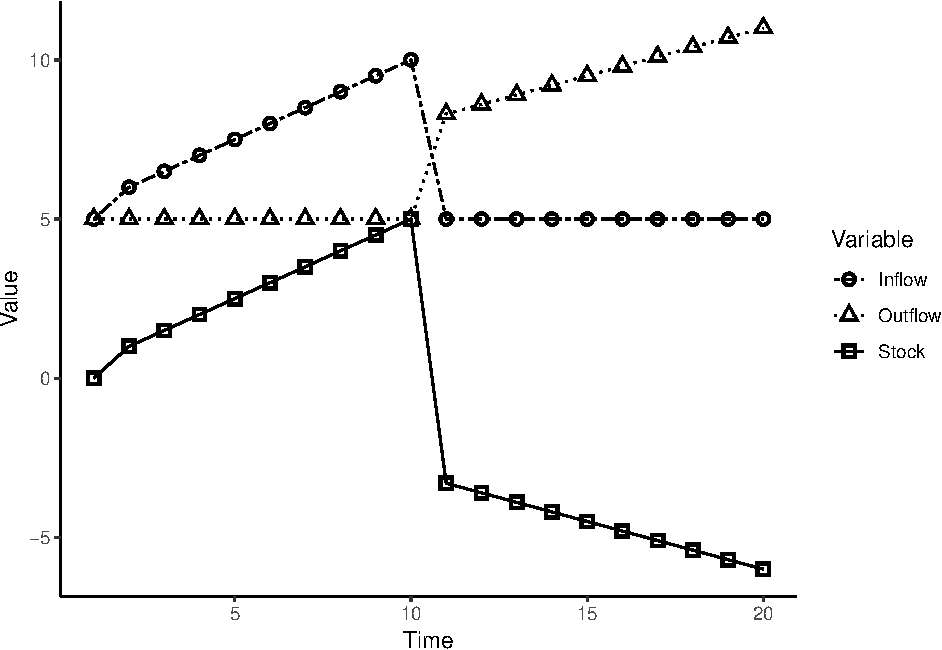
\includegraphics{figs/unnamed-chunk-5-1.pdf}
\caption{\label{fig:unnamed-chunk-5}the ol stock system\label{stocks}}
\end{figure}

\noindent Beginning at the first time point, inflows are equal to
outflows and the stock therefore sits at zero. Over the first ten time
points, however, outflows remain the same whereas inflows increase. With
inflows exceeding outflows the stock also increases up until time point
ten. At this time, inflows drop back down to five whereas outflows
increase -- leading to a large reduction in the stock. As outflows
continue to rise over time -- with no counterbalancing movement from the
inflow -- the stock ultimately decreases.

Systems theory uses stocks and flows as general labels for each of the
things in the system. Above, we described the behavior of the stocks and
flows with simple terms -- increasing, decreasing, or constant. Systems
theory also provides a more systematic way of describing trajectories
and explaining behavior over time. These are unpacked in an excellent
paper by Monge (1990), and the framework includes trend, magnitude, rate
of change, and periodicity. These are shown respectively in figure
\ref{monge}.

\begin{figure}
\centering
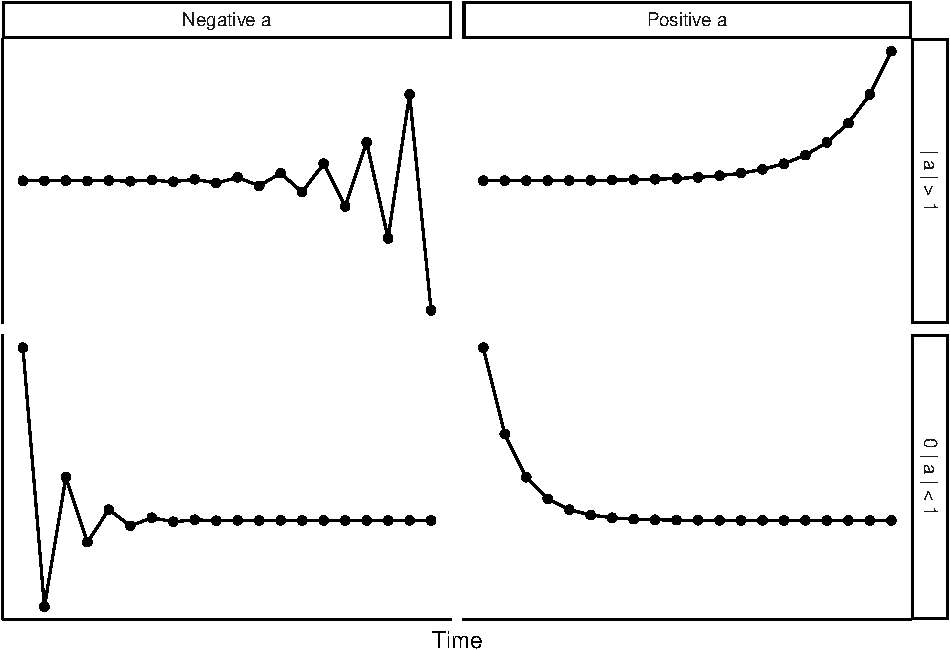
\includegraphics{figs/unnamed-chunk-6-1.pdf}
\caption{\label{fig:unnamed-chunk-6}monge image\label{monge}}
\end{figure}

\begin{center}

---------------

Insert Figure \ref{monge} Here

---------------

\end{center}

\hypertarget{trend}{%
\subsection{Trend}\label{trend}}

Dividing figure \ref{monge} into two portions -- the top and bottom --
reveals differences in trend. All of the panels on the top of the figure
have trend, whereas those on the bottom do not. Trend is the systematic
increase or decrease of a variable over time.

\hypertarget{magnitude}{%
\subsection{Magnitude}\label{magnitude}}

Magnitude is the level, value, or amount of the variable at each time
point -- the number on the \(y\) axis at each respective point in time.
For example, in panel \emph{C} of figure two the magnitude is low at
times 1, 2, and 3, but is high at later points in time. Additionally,
panel \emph{E} and \emph{F} have the same magnitude if we average their
values over time, but panel \emph{E} contains both high and low
magnitude, whereas the magnitude for the trajectory in panel \emph{F}
remains relatively constant.

\hypertarget{rate-of-change}{%
\subsection{Rate of Change}\label{rate-of-change}}

Monge refers to rate of change as \enquote{How fast the magnitude
increases or decreases per one unit of time.} Panels \emph{G} and
\emph{H} reveal differences in rates of change.

\hypertarget{periodicity}{%
\subsection{Periodicity}\label{periodicity}}

Periodicity is the amount of time before a pattern repeats itself, and
it is equivalent to the term cycle. The most important piece about
periodicity is that it must be couched with \enquote{controlling for
trend.} Notice that panel \emph{A} is periodic because, after
controlling for trend, there are repeated patterns over time.

\hypertarget{now-two-variables}{%
\subsection{Now two variables}\label{now-two-variables}}

It is of course possible to combine these notions when researchers are
studying processes with more than one variable. For example, a
researcher might describe the magnitude in their presumed dependent
variable with respect to the magnitude of their independent variable, or
the rates of change across the system of variables. When we turn to the
behavior and relationships among a system of variables a few additional
principles are available.

\hypertarget{lags}{%
\subsection{Lags}\label{lags}}

How long does it take for the presumed independent variable to produce
an effect on the outcome? This is the notion of lag.

\hypertarget{permanence}{%
\subsection{Permanence}\label{permanence}}

Once the effect happens, how long does it last?

\hypertarget{feedback-loops}{%
\subsection{Feedback Loops}\label{feedback-loops}}

Systems theory researchers often convey process by using feedback loops.
Feedback loops describe processes where a variable eventually relates
back to itself.

There are two common ways to describe the behavior of a focal variable
within a feedback loop. When feedback causes the variable to move in the
opposite direction than it initially moved, this is known as negative
feedback, deviation counteraction, or a balancing feedback loop
({\textbf{???}}; {\textbf{???}}). Here, an initial increase in \(x\)
leads to subsequent changes in the system that, through time, eventually
cause \(x\) to decrease. Now that \(x\) has gone down, more changes
happen in the system that, through time, eventually cause \(x\) to
increase.

When feedback, instead, causes the variable to move in the same
direction that it initially moved, this is known as postive feedback,
deviation ampliciation, or a reinforcing feedback loop ({\textbf{???}};
{\textbf{???}}). Here, changes in \(x\) in one direction lead to
eventual changes in \(x\) in the same direction and thus produce
exponential, explosive, or amplifying behavior. Of course, we can also
identify whether there is positive or negative feedback for every
variable in the system.

\hypertarget{example}{%
\subsection{Example}\label{example}}

People from our literature using these terms and principles to explain
something.

\hypertarget{summary}{%
\subsection{Summary}\label{summary}}

These systems theory notions are valuable tools to explain and describe
process. Note that we did not cover everything to keep the reading
concise and consistent. For example, ({\textbf{???}}) also covers
discontinuous systems, so please refer to his excellent paper for an
even deeper discussion. Now we turn to mathematics and statistics and
describe principles from these domains that are used to explain process.

\hypertarget{mathematical-statistical-and-dynamics-principles}{%
\section{Mathematical, Statistical and Dynamics
Principles}\label{mathematical-statistical-and-dynamics-principles}}

\hypertarget{difference-equations}{%
\subsection{Difference Equations}\label{difference-equations}}

In mathematics, a basic representation of a process over time is a
difference equation:

\begin{equation}
\label{basicD}
y_{t} = y_{t - 1}
\end{equation}

\noindent where \(y_{t}\) represents \(y\) now and \(y_{t-1}\) is the
variable at the prior time point. Here, the value of \(y\) is the same
at each \(t\), and the emergent behavior would be a flat line across
time. In systems theory terms, there would be no trend.

Although equation \ref{basicD} seems simple, it introduces a fundamental
concept in dynamics: memory. The variable now depends on where it was in
the past. It is constrained, there are boundaries on where it can go.

As we add terms to this basic difference equation the behavior of the
variable becomes more complex. Adding a forcing constant, \emph{c} in
equation \ref{basicD} produces positive or negative trend depending on
whether \emph{c} is, respectively, positive or negative. For example,
the following equation:

\begin{equation}
\begin{split}
\label{diffC}
y_{t} &= y_{t-1} + c \\ 
c &= -4
\end{split}
\end{equation}

\noindent produces a line that decreases by four units at each time
point.

The next level of complexity comes from autoregressive terms, which
represent the extent to which the variable relates to itself over time.
Here:

\begin{equation}
\begin{split}
\label{diffA}
y_{t} &= a y_{t-1} \\ 
a &= 0.5
\end{split}
\end{equation}

\noindent the variable is described over time but it does not retain the
same value at each \(t\). Instead, the variable is \emph{similar} over
time and the autoregressive term, \(a\), describes the extent of that
similarity. In equation \ref{diffA}, \(a\) is 0.5, meaning that the
relationship between the variable now and itself at the next time point
will be 0.5.

There are fundamental behaviors of dynamic variables based on their
autoregressive terms, and these are shown in figure \ref{dynamics_plot}.
The top row of figure \ref{dynamics_plot} shows the trajectory of
variables with autoregressive terms that are greater than one in
absolute value. These large terms produce explosive behavior --
exponential growth when \(a\) is positive and oscillating chaos when
\(a\) is negative. When the autoregressive term falls between zero and
one in absolute value, conversely, the variable converges to equilibrium
-- shown in the bottom two panels. Either the variable oscillates at a
decreasing rate until it reaches equilibrium (when \(a\) is negative) or
it converges there smoothly (when \(a\) is positive).

\begin{figure}
\centering
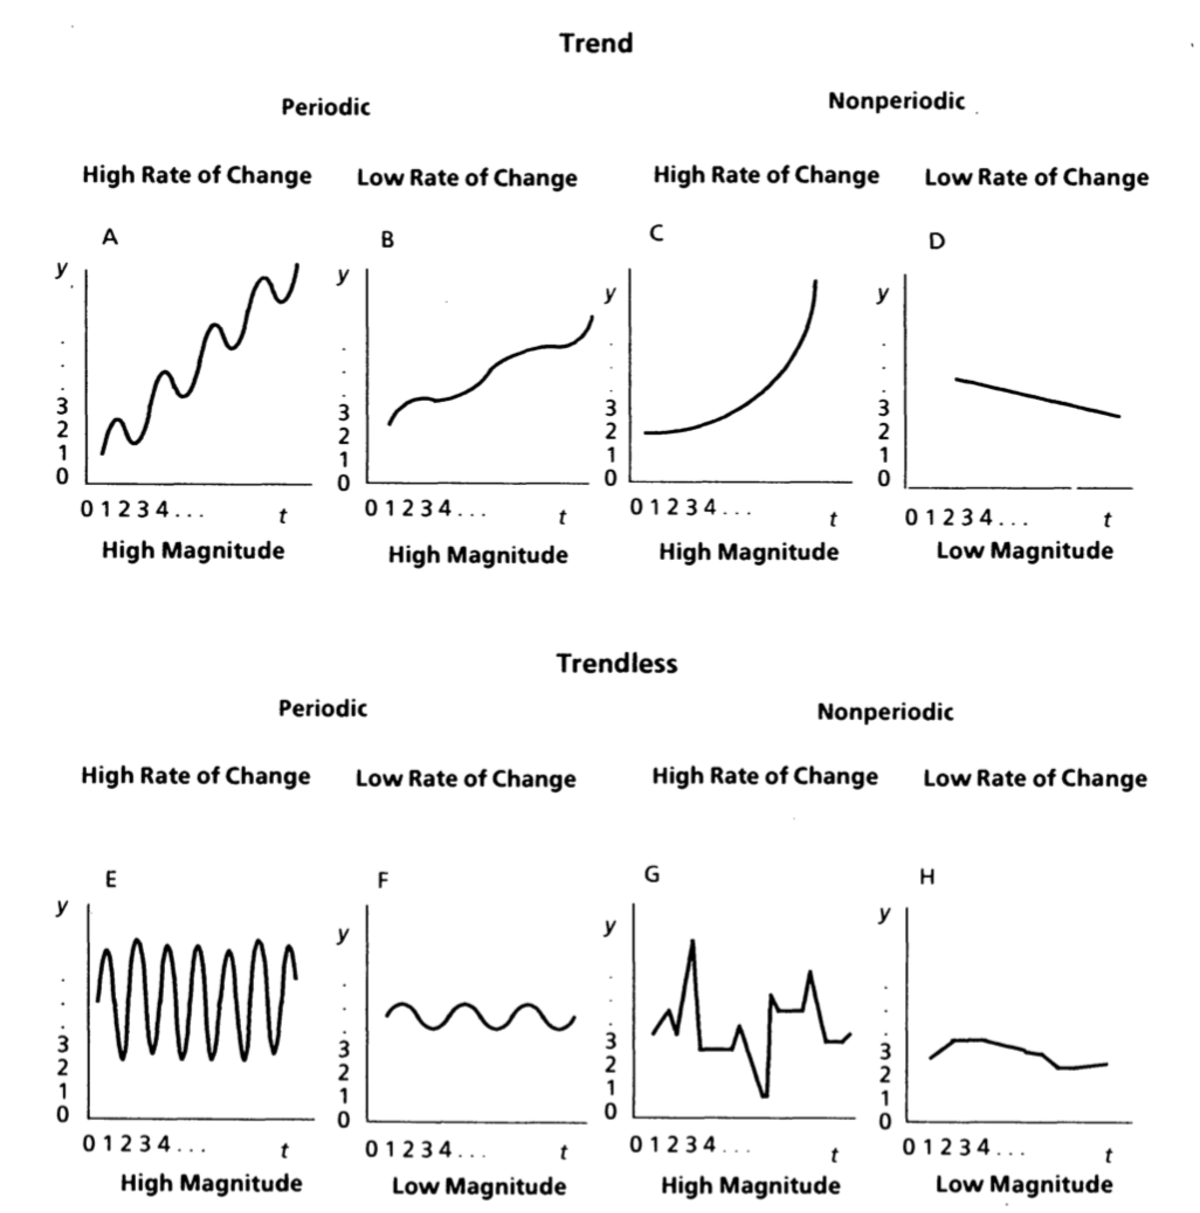
\includegraphics{figs/unnamed-chunk-7-1.pdf}
\caption{\label{fig:unnamed-chunk-7}dynamic equilibrium
fig\label{dynamics_plot}}
\end{figure}

\begin{center}

---------------

Insert Figure \ref{dynamics_plot} Here

---------------

\end{center}

\hypertarget{equilibrium}{%
\subsection{Equilibrium}\label{equilibrium}}

Equilibrium, then, describes the state of a variable that no longer
changes unless disturbed by an outside force. It can also be used to
describe multiple variable systems. In these contexts, equilibrium again
means that the state remains constant unless disturbed by an outside
force, but here state refers to the the entire system (i.e., all of the
variables). In \emph{static} equalibriums, the system has reached a
point of stability with no change, whereas \emph{dynamic} equilibrium
refers to systems with changes and fluctuations but no net change. That
is, the variables fluctuate across time in periodic ways but the general
state of the system does not diverge so as to change the behavior of the
entire system.

Predator-prey relationships are a typical example of a system in dynamic
equilibrium. For example, consider a predator-prey relationship between
bobcats and rabbits. As the rabbit population increases, the amount of
available food for the bobcats goes up. Over time, this raises the
population of the bobcats as well. Now with a greater bobcat population,
the rabbit population decreases because more are being killed. Over
time, this reduction in food opportunity decreases the bobcat
population. This back and forth oscillating pattern between variables
describes a dynamic equilibrium. The variables change and there may be
random disturbances to the system across time, but the net dynamics of
the system remain stable.

\hypertarget{system-of-equations}{%
\subsection{System of Equations}\label{system-of-equations}}

A difference equation with X influencing Y -- now I have lags
represented in math. A difference equation with X influencing Y and Y
influencing X -- now I have a feedback loop represented in a difference
equation. I may also get priodicity, trend, and equilibrium -- we could
work that out analytically but it is easier just to graph it.

Our route so far has been deterministic -- the mathematical
representations do not contain error. When we want to convey that the
underlying process -- the data generating mechanism -- contains error we
can consider a host of additional principles.

\hypertarget{stochastics}{%
\subsection{Stochastics}\label{stochastics}}

Stochastics, stated simply, refers to processes with error. Consider our
simple difference equation from above, adding an error component
produces:

\begin{equation}
\label{diffE}
y_{t} = a y_{t-1} + c + e_{t}
\end{equation}

\noindent where all terms are defined above but \(e_{t}\) represents an
error term that is incorporated into \(y\) at each time point. Errors
cause \(y\) to be higher or lower at specific points in time than we
would have expected given a deterministic process. For example, at time
\(t\) the error might push \(y\) to a higher value, and at \(t+1\) to a
lower value. Errors are therefore said to be random because we cannot
predict their value at any specific \(t\). In aggregation (i.e.,
averaged across time), however, positive errors cancel negative errors,
and large errors are less likely than small errors. Any time we have an
accumulation of random error we get a normal distribution
({\textbf{???}}). In stochastic systems, therefore, the errors are said
to be distributed \(N(0, 1)\) -- that is, random and unpredictable at
any specific \(t\) but distributed with certain constraints across time.

It can also be helpful to think about what error is not. Anything that
is systematic, predictable, or common (using those in layman's terms)
cannot be error -- leaving error to be the random \enquote{left overs.}
An aggregation of randomness is a normal distribution.

\hypertarget{white-noise-and-random-walks}{%
\subsection{White Noise and Random
Walks}\label{white-noise-and-random-walks}}

There are two fundamental stochastic processes: white noise and random
walks. White noise is a process that only has error. Setting \emph{c}
and \emph{a} to zero in equation \ref{diffE} produces a white noise
process.

\begin{equation}
\begin{split}
\label{whitenoise}
y_{t} &= a y_{t-1} + c + e_{t} \\
a &= 0 \\
c &= 0
\end{split}
\end{equation}

\noindent Here, all we have is error over time. Panel \enquote{A} of
figure \ref{noise} shows the behavior of a white noise process over
time. Random walks are similar, but \emph{a} is now equal to one.

\begin{equation}
\begin{split}
\label{rw}
y_{t} &= a y_{t-1} + c + e_{t} \\ 
a &= 1 \\ 
c &= 0
\end{split}
\end{equation}

\noindent This representation is also an error process, but there is
self-similarity across time. Panel \enquote{B} of figure \ref{noise}
presents a random walk. Although random walks can sometimes appear to be
moving in a systematic direction, ultimately their behavior is
unpreditable: they could go up or down at any moment.

Random walks and white noise are error processes over time. White noise
processes fluctuate randomly, whereas random walks fluctuate randomly
while retaining some self-similarity through time. These two principles
are the null hypotheses of time-series analysis in econometrics -- where
the first task in a longitudinal study is to demonstrate that you are
investigating something that is not a random walk or white noise.

\begin{figure}
\centering
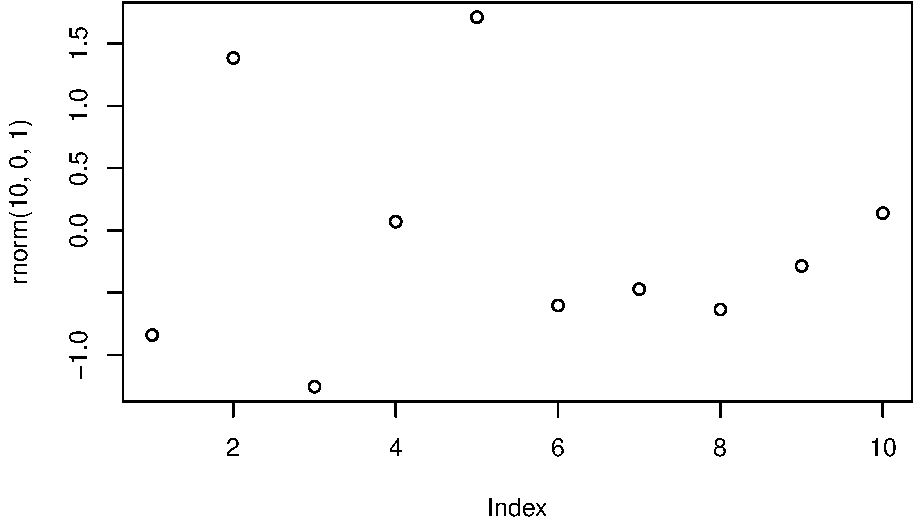
\includegraphics{figs/unnamed-chunk-8-1.pdf}
\caption{\label{fig:unnamed-chunk-8}this one will be a white noise process
and a random walk\label{noise}}
\end{figure}

Now that we have added the conept of error our focus changes from the
exact values of variables over time to their distributions.

\hypertarget{stationary}{%
\subsection{Stationary}\label{stationary}}

Stationary is a term that describes the properties of a process. If a
process is stationary, its mean and variance are stable -- they are
similar across all \(t\). In simple terms, this means that we expect the
properties (mean and variance) of a time series at time \(t\) to be the
same at time \(t+1\).

\hypertarget{cointegration-and-granger-causality}{%
\subsection{Cointegration and Granger
Causality}\label{cointegration-and-granger-causality}}

\hypertarget{example-dishop-maybe-denrell}{%
\subsection{Example: Dishop (maybe);
Denrell}\label{example-dishop-maybe-denrell}}

People from our literature using these principles to explain something.

\hypertarget{summary-1}{%
\subsection{Summary}\label{summary-1}}

\hypertarget{computational-principles}{%
\section{Computational Principles}\label{computational-principles}}

Above, we described and explained behavior over time by using
representations most people are familiar with: verbal descriptions,
plots, and math. There has recently been a push to comp model. These
people are trying to do the same thing, but represent their process in a
computer.

Think of it this way. Above, we represented process with graphs,
equations, and terms. To do so required certain principles. When we want
to describe something in a computer language we also need certain
principles: certain requirements or fundamentals about how we explain
the process.

Vancouver has pointed out some of these. He framed them as difficult
pieces to putting stuff into code.

\hypertarget{key-states}{%
\subsection{Key States}\label{key-states}}

What are the important states? A variable is an entity that can take
different values at one point in time. A state is a variable that
fluctuates over time. In information technology and computer science, a
program is described as stateful if it is designed to remember preceding
events or user interactions; the remembered information is called the
state of the system.

We can also talk about the global state of the system as a whole -- its
cumulative form. The state of the \emph{system} describes enough about
the system to determine its future behavior in the absence of any
external forces affecting the system. The set of possible combinations
of state variables is called the state space of a system.

\hypertarget{state-dynamics}{%
\subsection{State Dynamics}\label{state-dynamics}}

\hypertarget{constants}{%
\subsection{Constants}\label{constants}}

Values that do not change over time. Usually constants occur in the
coefficients, or the weights. Vancouver's comp model 2018 included a
weight relating assigned goal difficulty and goal specificity to
self-efficacy that did not change over time.

\hypertarget{actions}{%
\subsection{Actions}\label{actions}}

\hypertarget{action-selection}{%
\subsection{Action selection}\label{action-selection}}

\hypertarget{contextenvironment}{%
\subsection{Context/Environment}\label{contextenvironment}}

How is the process situated? Simon's mouse behavior environment. He
defines the context in which it can move around. Things happen with
respect to the environment.

\hypertarget{noise}{%
\subsection{Noise}\label{noise}}

Is there error in the system, if so, where?

\hypertarget{time-scale}{%
\subsection{Time Scale}\label{time-scale}}

How long does the process operate for? How many iterations does my for
loop go for?

\hypertarget{example-simon-1956}{%
\subsection{Example: Simon 1956}\label{example-simon-1956}}

\hypertarget{key-states-1}{%
\subsubsection{key states:}\label{key-states-1}}

\begin{itemize}
\tightlist
\item
  hunger and thirst
\item
  It is easier to think of these as stocks: food and water.
\end{itemize}

\hypertarget{state-dynamics-1}{%
\subsubsection{State dynamics:}\label{state-dynamics-1}}

\begin{itemize}
\tightlist
\item
  The body requires energy, so the food and water stocks decrease over
  time (i.e., hunger and thirst increase)
\end{itemize}

\hypertarget{actions-1}{%
\subsubsection{Actions}\label{actions-1}}

\begin{itemize}
\item
  these actions satisfy the state dynamics

  \begin{itemize}
  \tightlist
  \item
    resting, exploration, goal striving
  \end{itemize}
\end{itemize}

\hypertarget{action-selection-1}{%
\subsubsection{Action selection}\label{action-selection-1}}

\begin{itemize}
\item
  If the food and water stocks are above threshold, the agent rests
\item
  When the stock of any need dips below threshold, the agent explores
\item
  During exploration

  \begin{itemize}
  \tightlist
  \item
    agent randomly runs into objects. If they encounter a single object
    relevant to one of the needs, the agent acquires it
  \item
    If the agent encounters two or more need-relevant objects, they
    evoke a simple ratio to make a decision

    \begin{itemize}
    \tightlist
    \item
      compare energy required to meet the need (M) to the storage
      capacity with respect to the need (S)
    \item
      or the effort required to get the object to how large the stock
      for this need is. Super large stocks take precedence
    \end{itemize}
  \end{itemize}
\end{itemize}

\hypertarget{environment}{%
\subsubsection{Environment}\label{environment}}

\begin{itemize}
\tightlist
\item
  a space with goals within which the entity moves
\item
  the individual is located in an environment that contains spatially
  distributed goal-relevant objects such as sources of food and water
  (239).
\item
  the size of the food and water stocks are determined by the
  availability of the resources in the environment. Water is easier to
  come by than food and so food storage requirements are greater.
  Similarly, breathable air is easier to obtain than water and so its
  storage requirements are less than both food and water (239).
\end{itemize}

\hypertarget{summary-2}{%
\subsection{Summary}\label{summary-2}}

\newpage

\hypertarget{references}{%
\section{References}\label{references}}

\setlength{\parindent}{-0.5in}
\setlength{\leftskip}{0.5in}


\end{document}
